\section{Architecture}

\subsection{Matching}

Aufgabe eines \textit{Matchers} ist es, die korrespondierenden Elemente aus Modell A und Modell B, also die Elemente, die in beiden Modellen übereinstimmen, zu identifizieren.
Dabei ist das Ergebnis vor allem davon abhängig anhand welcher Kriterien der Matcher eine Übereinstimmung festlegt.
Hier wird unter anderem unterschieden zwischen \textit{ID-}, \textit{signatur-} und \textit{ähnlichkeitsbasierten} Verfahren.\\
Das Framework definiert einen Extension Point (siehe \ref{exp:org.sidiff.matcher.extensionpoint}), um durch entsprechende Matcher erweitert werden zu können.
Die konzeptuelle Struktur des Ergebnisses, also eines \textit{Matchings}, ist durch das in Abbildung \ref{fig:matching_model} dargestellte, EMF-basierte Metamodell definiert.

\begin{figure}[h!]
\centering
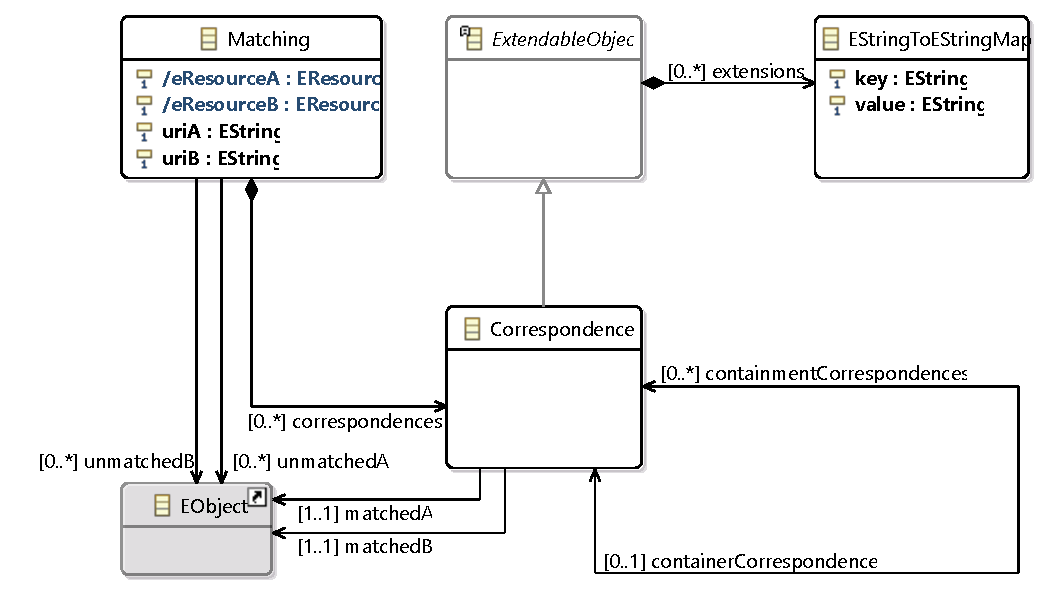
\includegraphics[width=0.75\textwidth]{images/architecture/matching_model}
\caption{Abstract Syntax of a model matching}
\label{fig:matching_model}
\end{figure}

TODO: Beschreibung der abstrakten Syntax

\newpage


\subsection{Difference Derivation}
Ausgehend von den gefunden Korrespondenzen berechnet der \textit{Difference Derivator} eine technische Differenz (\textit{low-level difference}) der Mo\-del\-le.
Alle Objekte und Referenzen, für die keine Korrespondenz existiert, müssen demnach entweder in Modell B hinzugefügt, oder aus Modell A entfernt worden sein. 
Durch die Verwendung eines \textit{Technical Difference Builders} können Modellelemente von der Differenzberechnung ausgeschlossen werden.
Dieser kann ebenfalls über einen Extension Point (siehe \ref{exp:org.sidiff.difference.technical.extensionpoint}) erweitert und für die jeweilige Domäne angepasst werden.
\newpage


\subsection{Lifting Engine}

Aufgabe der \textit{Lifting Engine} ist es, die zuvor berechnete technische Differenz semantisch zu liften.
Eine technische Differenz enthält alle Än\-der\-ung\-en  auf Basis des Metamodells, also der abstrakten Syntax.
Beim \textit{semantischen liften} werden die einzelnen Änderungen zu sogenannten \textit{Semantic Change Sets} gruppiert, welche Editieroperation auf Ebene der konkreten Syntax repräsentieren.\\
Die konzeptuelle Struktur einer gelifteten, symmetrischen Differenz ist durch das in Abbildung \ref{fig:symmetric_model} dargestellte, EMF-basierte Metamodell definiert. 

\begin{figure}[h!]
\centering
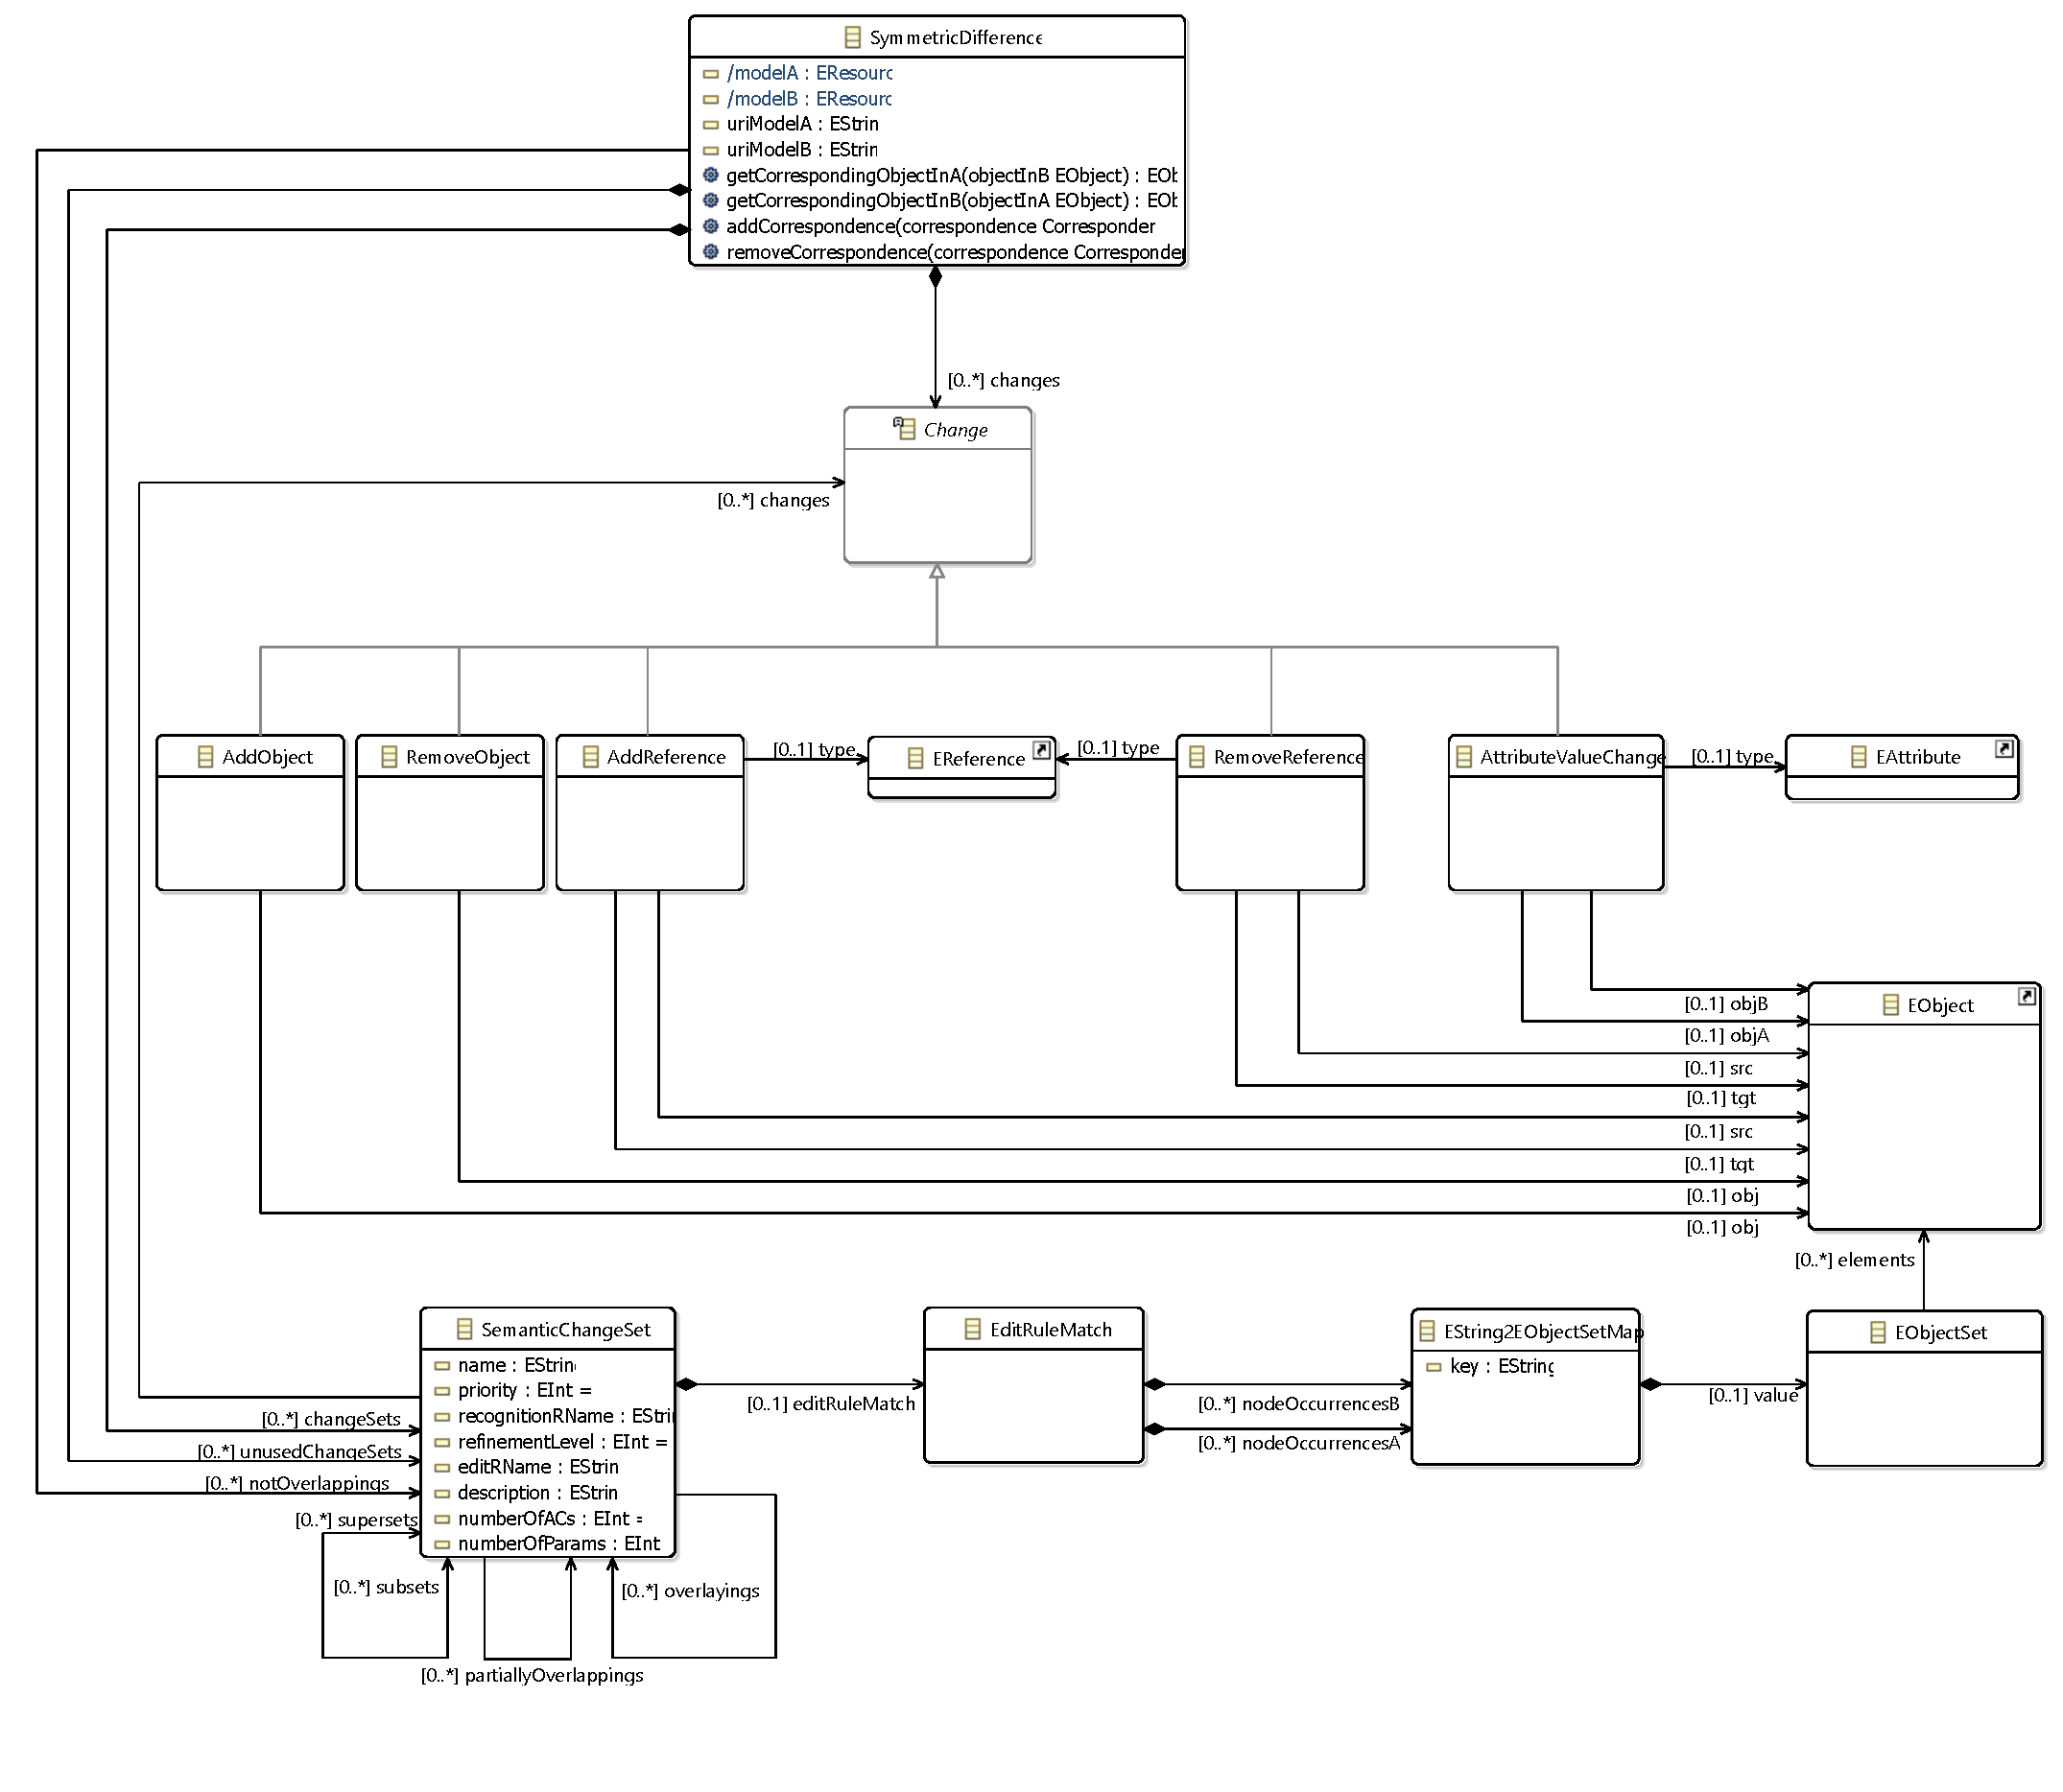
\includegraphics[width=\textwidth]{images/architecture/symmetric_model}
\caption{Abstract Syntax of a descriptive model difference}
\label{fig:symmetric_model}
\end{figure}


\begin{figure}[h!]
\centering
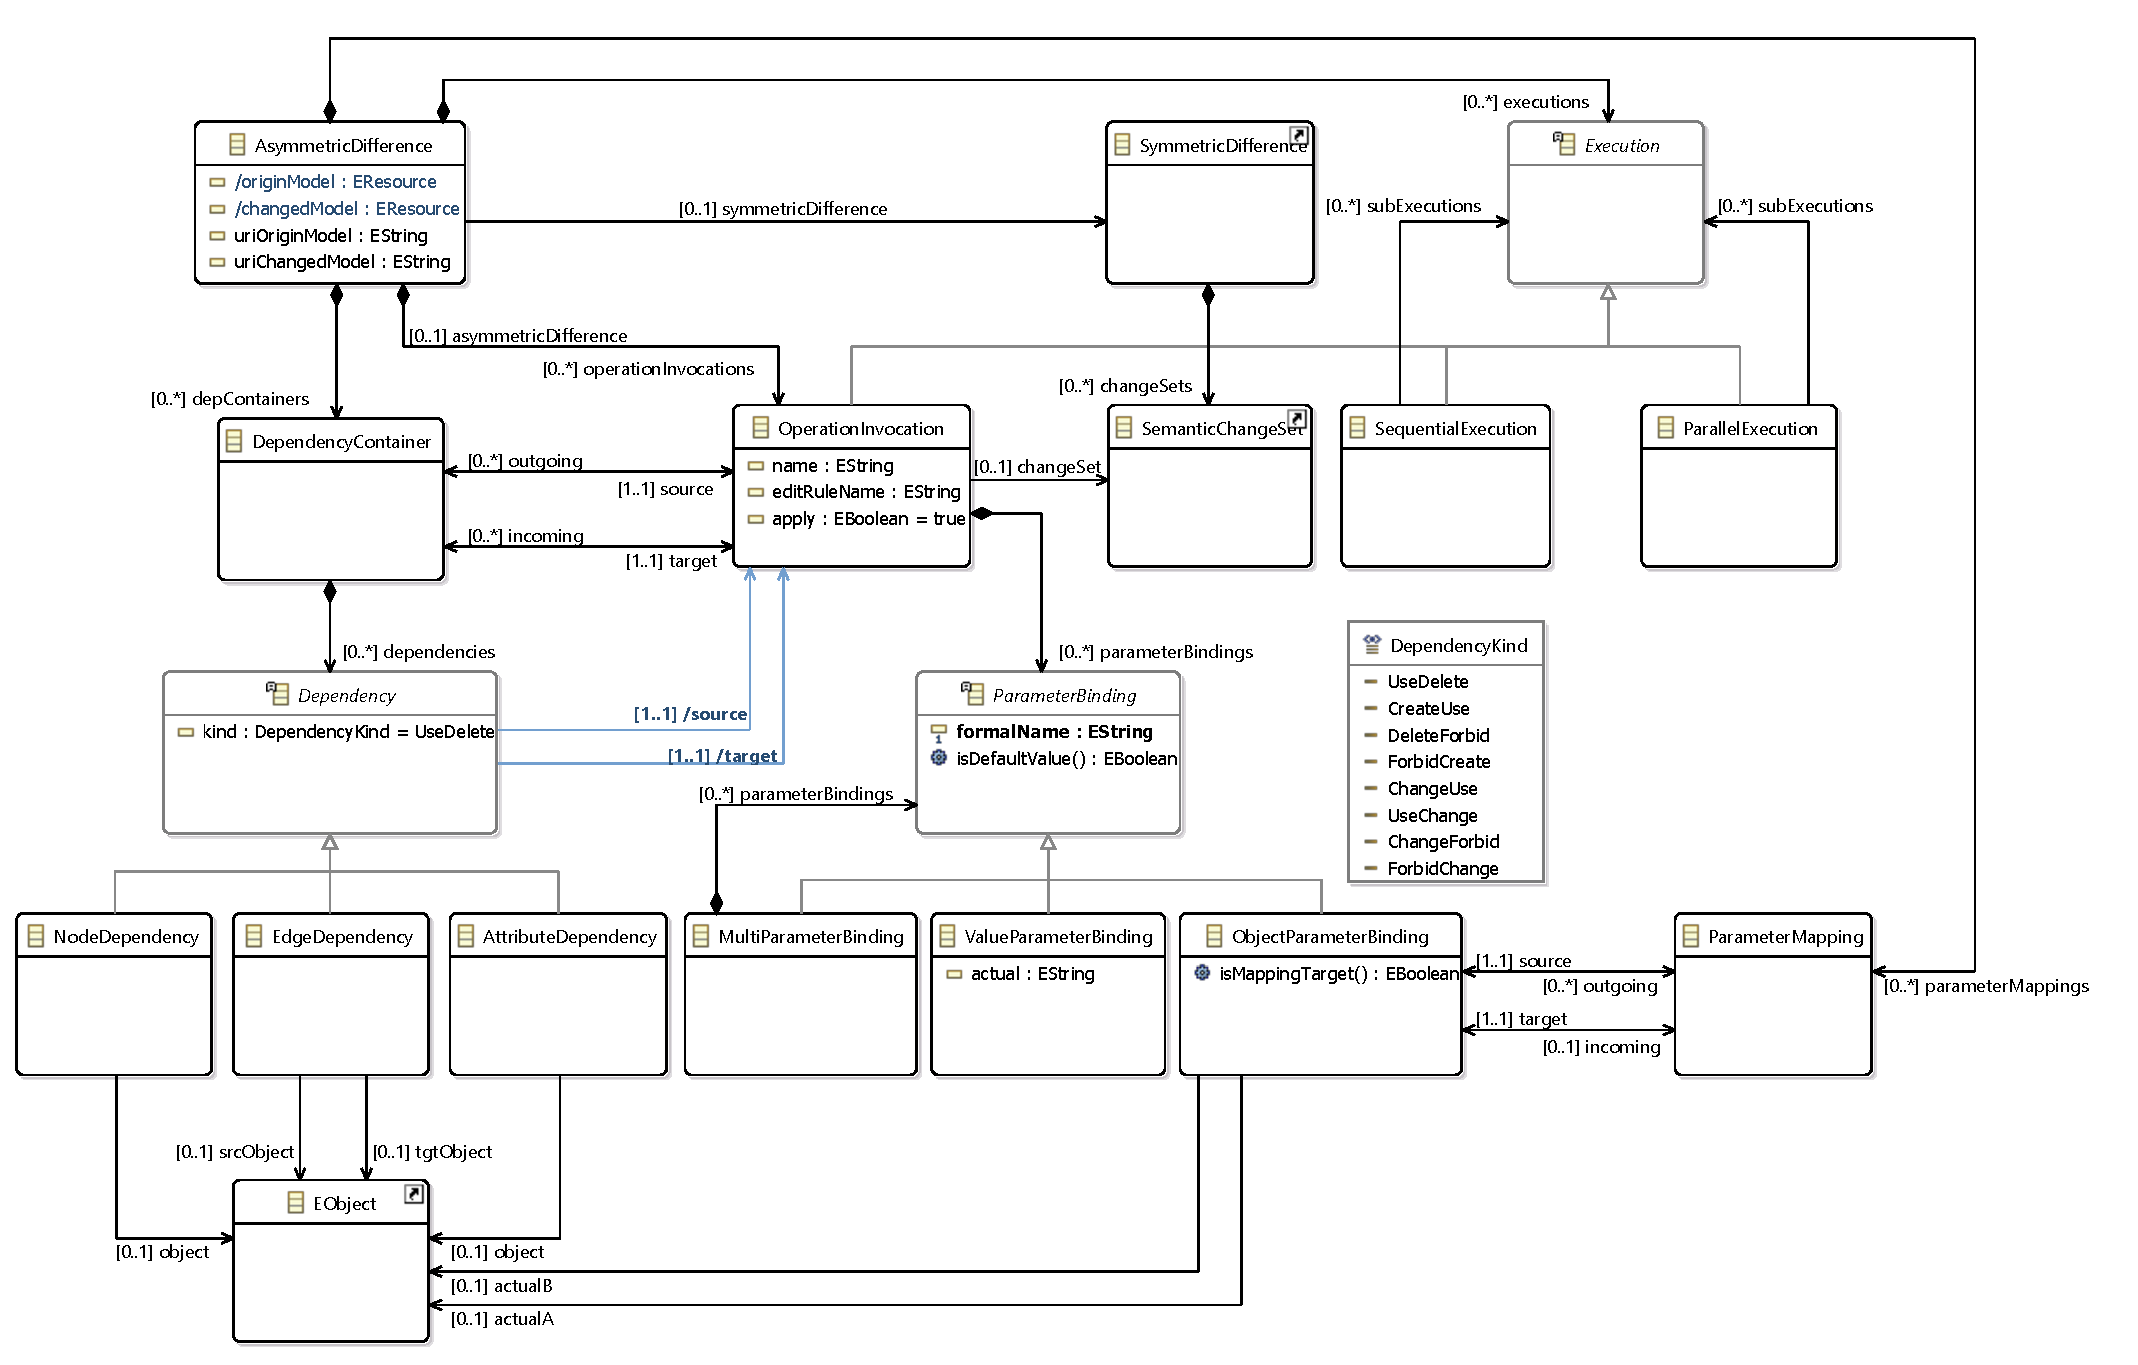
\includegraphics[width=\textwidth]{images/architecture/asymmetric_model}
\caption{Abstract Syntax of a prescriptive model difference}
\end{figure}

\newpage


\subsection{Rule Base}

\begin{figure}[h!]
\centering
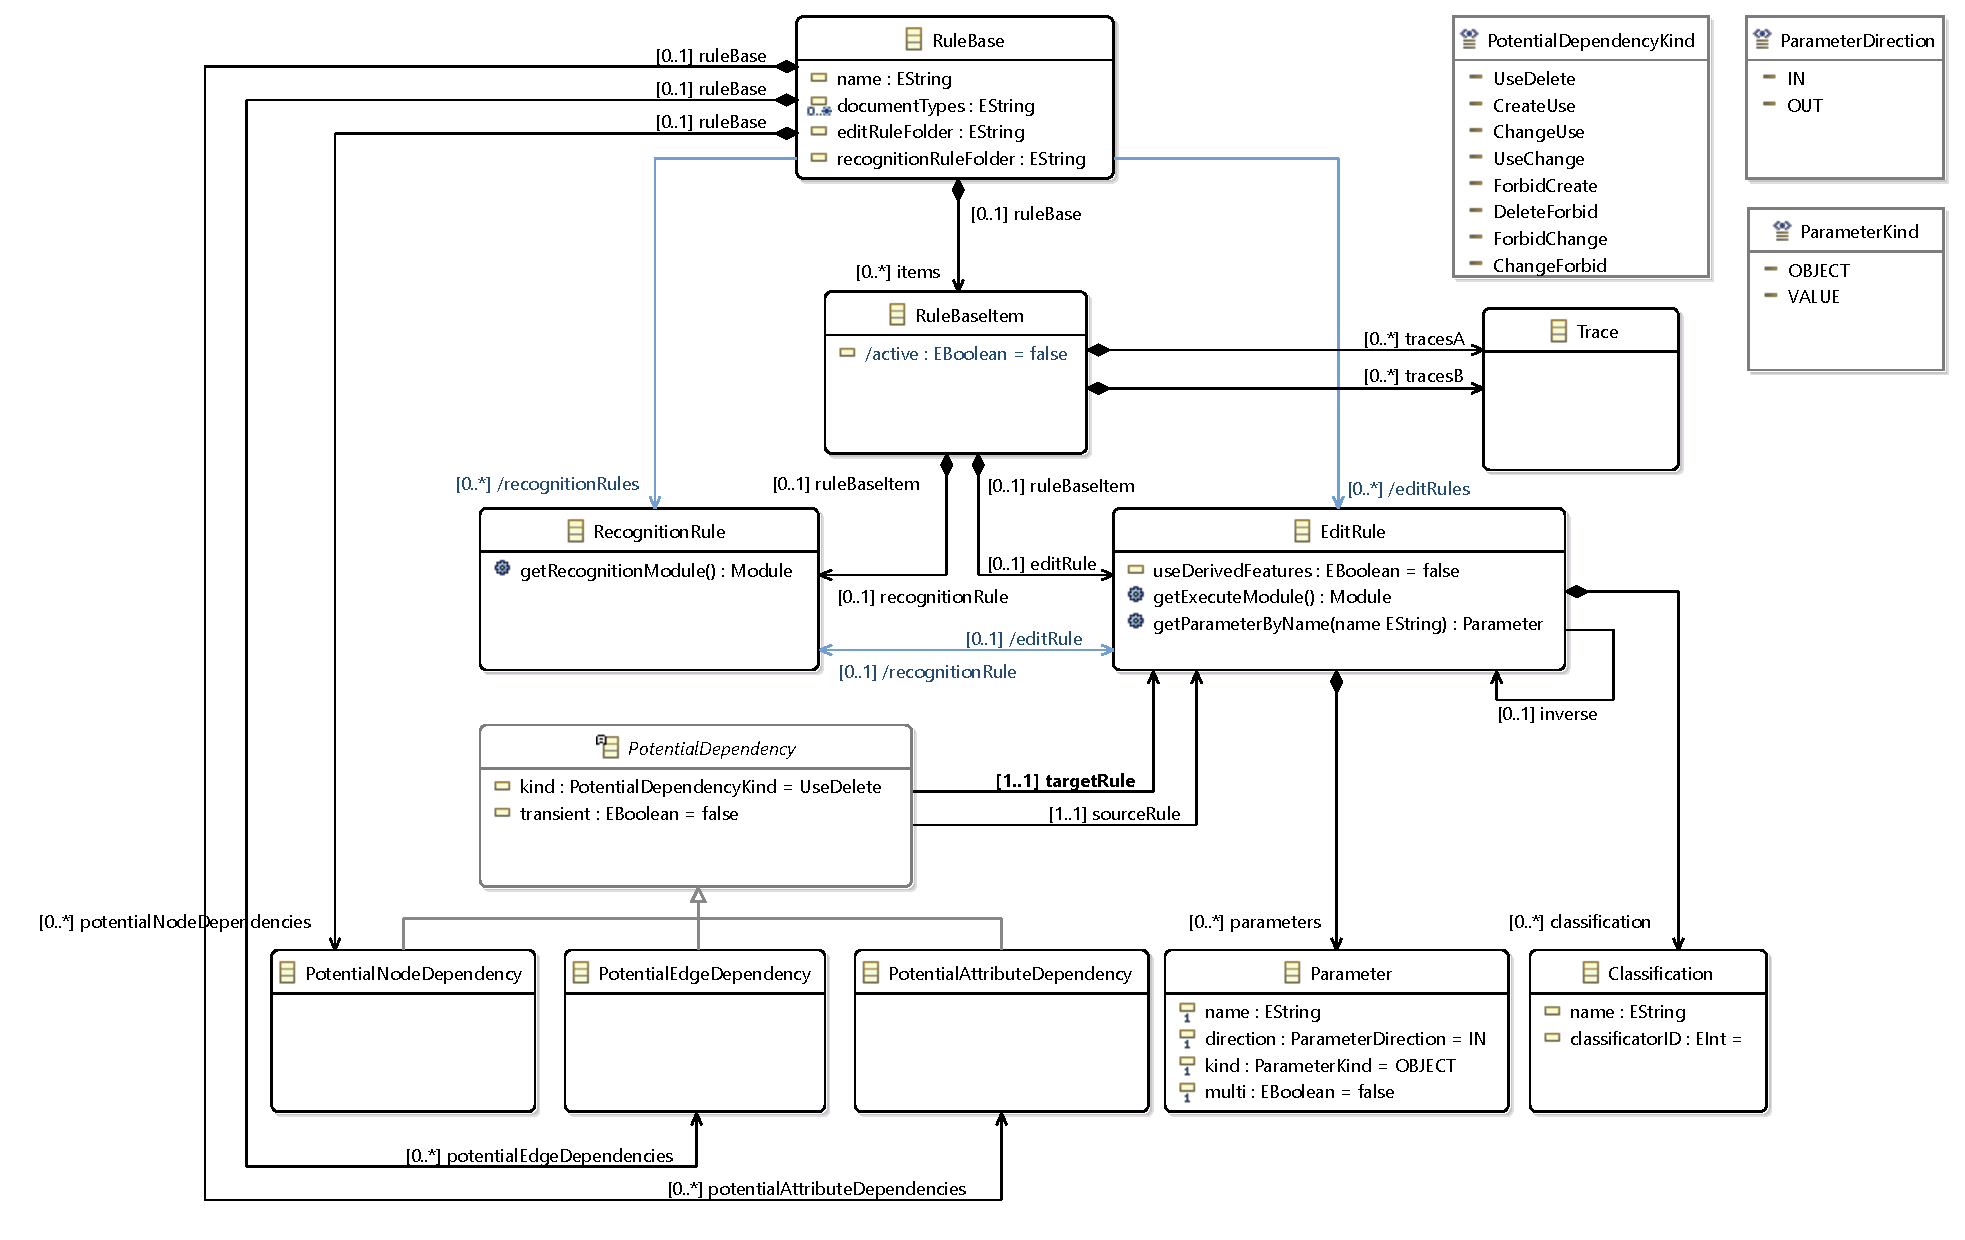
\includegraphics[width=\textwidth]{images/architecture/rulebase_model}
\caption{Conceptual structure of a rule base}
\end{figure}


